%!TEX root = ../Thesis.tex

\chapter{Evaluation and optimization}
	During the course of creating the application we tried different approaches to several interim steps. In this chapter we discuss how using different algorithms yielded different results.

	\section{Dataset}
	In order to test and optimize our detector we created a set of 101 images and annotated them manually with the following information: each intersection on the board was marked with a point, either as an empty intersection, an intersection with a white piece on it or one occupied by a black piece. Also, the location of all pieces was marked with a circle, i.e. with a center and its approximate radius.

	To have an image set that covers as many possible game situations as possible we took pictures in three different lighting conditions and on different backgrounds. Each time we took images of an empty board without any pieces, a board with only some few images and a configuration as it often happens during endgame. That is, many pieces on the board and lots of them in a line.

	Each board configuration was photographed from different angles in $\varphi$ (azimuth) and $\theta$ (polar) direction and from two directions, i.e. facing the board from the side a player would and rotated by 90\textdegree~ as a third person would see the board.

	\begin{figure}
		\begin{subfigure}[b]{0.3\textwidth}
			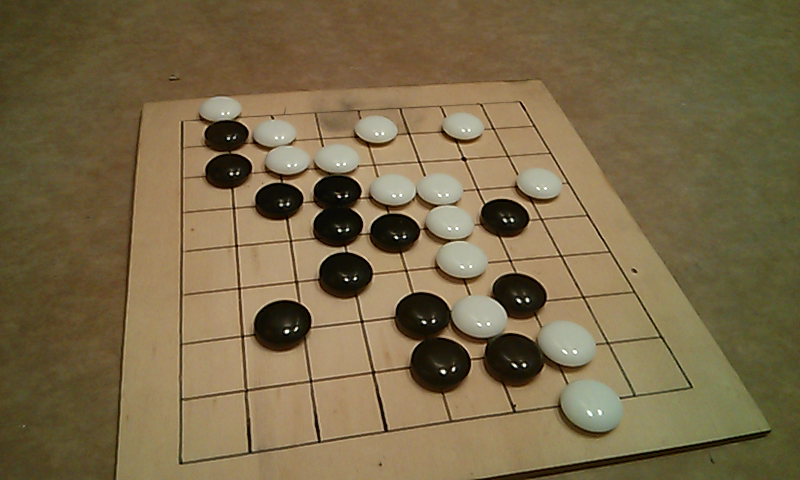
\includegraphics[width=\textwidth]{images/warmLight_many_leftMedium.png}
			\caption{Paper in warm light; camera left on medium height}
		\end{subfigure}
		~
		\begin{subfigure}[b]{0.3\textwidth}
				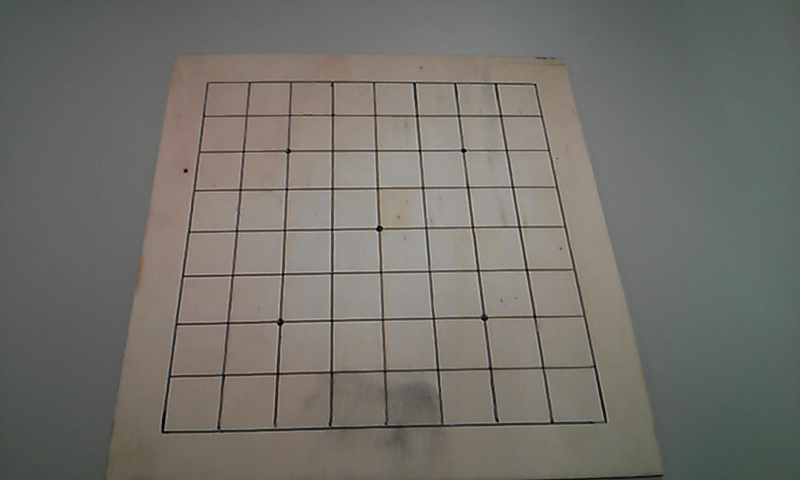
\includegraphics[width=\textwidth]{images/neonDesk_empty_centerAbove.png}
				\caption{Plain gray desk in neon light; camera centered high}
		\end{subfigure}
		~
		\begin{subfigure}[b]{0.3\textwidth}
				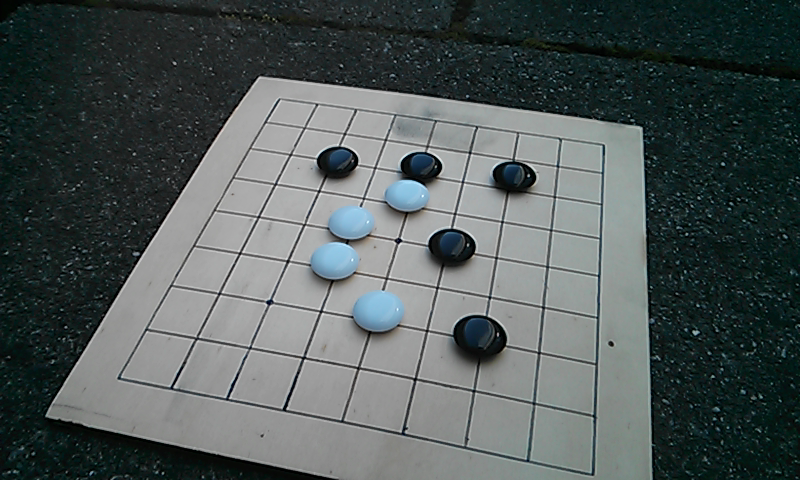
\includegraphics[width=\textwidth]{images/shadowStone_some_rightAbove.png}
				\caption{Dark stone surface in the shadow; camera right high}
		\end{subfigure}
		\\
		\begin{subfigure}[b]{0.3\textwidth}
				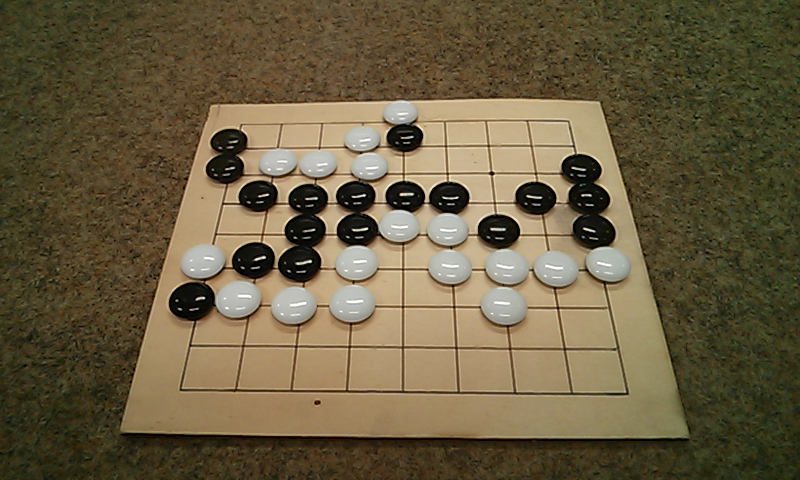
\includegraphics[width=\textwidth]{images/neonFloor_many_centerLow.png}
				\caption{Brown carpet in neon light; camera centered low}
		\end{subfigure}
		~
		\begin{subfigure}[b]{0.3\textwidth}
				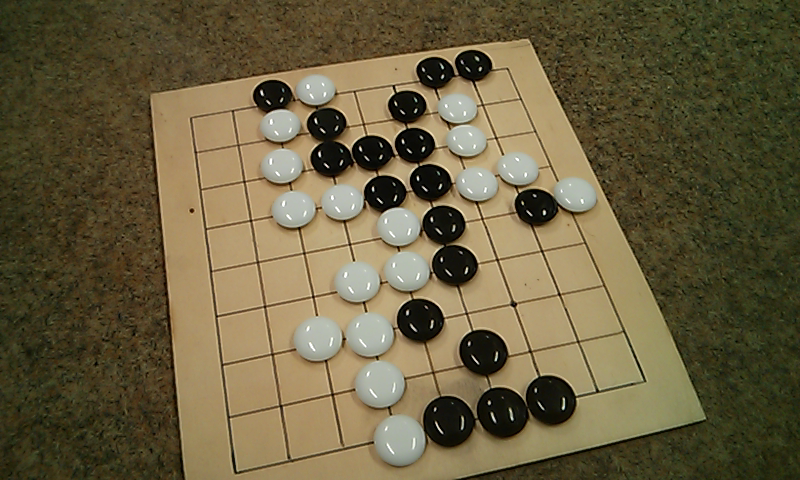
\includegraphics[width=\textwidth]{images/neonFloor_many_centerLow_rotated.png}
				\caption{Like (d) but from bystanders'	 perspective}
		\end{subfigure}
		~
		\begin{subfigure}[b]{0.3\textwidth}
			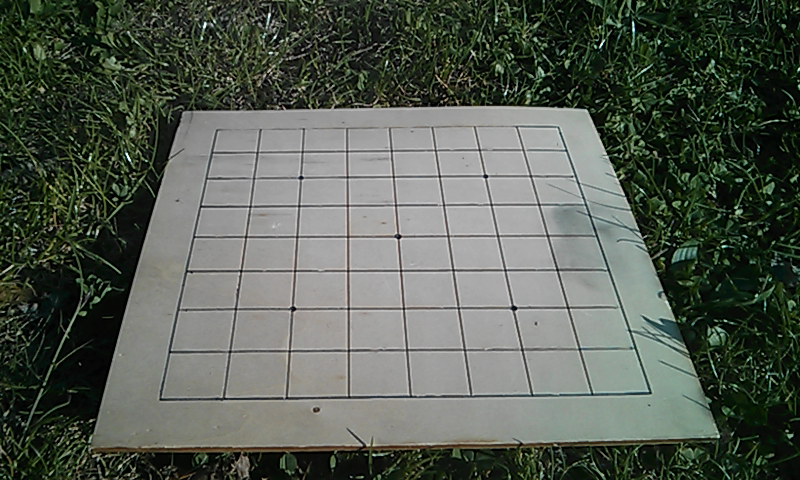
\includegraphics[width=\textwidth]{images/sunnyGrass_empty_centerLow.png}
			\caption{On grass in sunlight; camera centered low}
		\end{subfigure}

		\caption{Some examples of different ligthing conditions, angles and backgrounds as well as different piece count}
	\end{figure}

	We ended up with: 29 images taken in cold neon light on a plain gray desk; 26 images taken in the same light on a textured, brown carpet; 25 images taken on a sunny day in the shadow on a stone surface; 17 images in warm artificial light on a textured paper background. Furthermore we have 5 images taken in the sun on an evening in which the board lay in grass.

	The images were taken by starting the app normally but then instead of starting detection saving the input image on the internal memory of the device. While in the beginning we saved images to png we later switched to persisting the images into yml format and retake the previous images. This has the advantage that we can be absolutely sure that the input to our test instances are the same as they would be on a phone, as no png coding and decoding takes place. Also we had problems in the beginning because OpenCV's image persisting function presumably does not recognize that the camera image is encoded in RGB (see \ref{android-detector}), which lead to different results on our desktop hardware than on our Android phone.

	31 of the images were randomly chosen as a test set evenly spread over all lighting conditions as well as piece and angle configurations. The grass images were not part of the test set as they soon turned out to be very difficult. We included them in the training set, though. This set was used to improve our detector.

	To do so we assumed that there is a global maximum for the overall quality of results when adjusting parameters of the used algorithms. Even if this assumption were wrong we optimized for a local maximum. Then we tried manually to find roughly the optimal parameters for some randomly chosen images for every algorithm. Finally we adjusted them automatedly by brute forcely trying every combination of parameters in the vicinity of the manually chosen on every image on a cluster of 45 oktacore machines and checking the results against the annotations.

	\section{Visible intersections}
	When evaluating the detection rate of visible intersections we first checked if the intersection was within the boundaries of the annotated board and a padding of 15 pixels. If not the intersection was considered uninteresting and did neither count positively nor negatively. If it was inside the board we searched the nearest annotated intersection for every detected one. If there was none within a range of 15 pixels the intersection was counted as a false positive. But if there was, then the annotated intersection was marked as detected and not considered as a possible match for other intersections. The threshold was chosen roughly as a quarter of the average distance between two intersections and a third of the diameter of a piece as measured in some sample images.

	In the end we measured the quality of the algorithm as the ratio of detected to undetected intersections while also considering the number of false positives.

	\subsection{HOUGH}
	%todo
	\subsection{LSD}
	%todo
	\subsection{FAST}
	%todo

	\section{Occluded intersections}
	\subsection{Contours}
	\subsection{Hough}

	\section{Vorverarbeitung}
	\subsection{Gauss}
	\subsection{Informationen aus vorherigem Run}
